\section{Background \& Motivation}
\begin{frame}{Background \& Motivation}
\begin{block}{Background}
\begin{itemize}
    \item Anomaly detection is crucial in domains like manufacturing, healthcare, and surveillance.
    \item PatchCore is a strong unsupervised method of this field using:
    \begin{itemize}
        \item CNN backbone to extract patch features
        \item Coreset sampling + nearest neighbor search for anomaly scoring and visualize anomalous regions on given image
    \end{itemize}
\end{itemize}
\end{block}
\begin{figure}
    \centering
    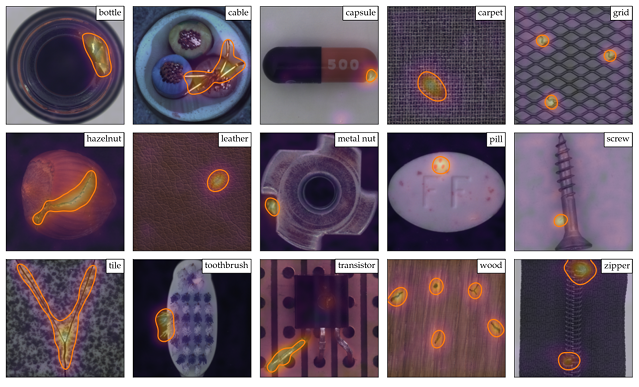
\includegraphics[width=0.3\linewidth]{intro.png}
    \caption{Segmentation results from PatchCore}
\end{figure}
\end{frame}
\begin{frame}{Background \& Motivation}
\begin{block}{Motivation}
    \begin{itemize}
        \item Despite the effectiveness of PatchCore method in anomaly dection field, its CNN encoder's backbone appears to lack several features to perform better in real-life detection like semantic understanding or global feature focus.
        \item Therefore, replacing PatchCore’s CNN backbone with a VLM encoder is a remarkable extension to utilize this state-of-art model in not only anomaly detection but also other aspects requiring VLMs.
    \end{itemize}
\end{block}
\end{frame}